% !TEX root = ../main.tex
\section{Data} \label{sec:data}
The performance of video generation models is inextricably linked to the scale, quality, and diversity of their training data.
However, naively scaling up data collection yields diminishing returns and is often bottlenecked by practical factors such as acquisition costs and computational overhead.
To address these challenges, we have developed an integrated and scalable data infrastructure built through several synergistic modules.
The \textbf{Data Profiling Engine} extracts multi-dimensional attributes for each sample---covering structural, semantic, motion, camera, and quality aspects---providing a unified foundation for downstream processing.
The \textbf{World-Knowledge Topological Graph} organizes visual concepts into a hierarchical semantic structure, enabling distribution-aware sampling and enhancing long-tail coverage.
The \textbf{Dense Structured Captioning} module generates hierarchical textual descriptions to provide fine-grained semantic supervision, while a complementary \textbf{Caption Rewriter} maps brief user prompts into this same structured format during inference, thereby closing the prompt distribution gap between training and deployment.
Building upon this infrastructure, we organize the curated corpus into a stage-wise \textbf{Data Curriculum} (\cref{subsec:data_curriculum}), which governs the volume and composition of data consumed during each phase of progressive pre-training (\cref{sec:training}).

\subsection{Data Profiling Engine}
The Data Profiling Engine converts raw multimodal samples into structured, multi-dimensional records that capture structural, semantic, motion, camera, and quality attributes. Rather than relying on free-form annotations, we project every sample onto a fixed schema, providing a unified and queryable representation for heterogeneous image and video data. These standardized records drive all subsequent processing stages, from filtering and sampling to captioning. The core annotations are generated by powerful vision--language models (VLMs), further augmented by a suite of specialized scoring and detection models detailed below.~\cref{fig:profiling_engine} provides an overview of this pipeline.

\begin{figure}[t]
\centering
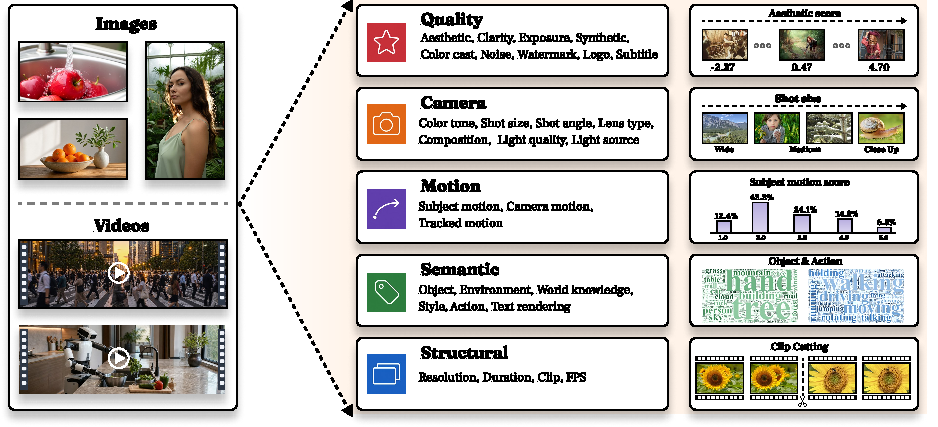
\includegraphics[width=\linewidth]{figures/data_profiling_engine/data_profiling_engine.pdf}
\caption{\textbf{Overview of the Data Profiling Engine.} Each image or video sample is annotated across five complementary dimensions (structural, semantic, motion, camera, and quality) into a structured profile record, which then drives downstream filtering, balanced sampling, and captioning.}
\label{fig:profiling_engine}
\end{figure}

\noindent\textbf{Structural Metadata.}
This dimension records fundamental media attributes, including spatial resolution, native frame rate, and duration. For video content, we employ TransNetV2~\cite{soucek2024transnet} to detect shot boundaries and segment the video stream into clip-level units, ensuring that each training clip represents a single, temporally coherent shot.

\noindent\textbf{Semantic Labels.}
Each sample is assigned semantic annotations along with category-level confidence scores, which serve as the foundation for the World-Knowledge Topological Graph used during distribution-aware sampling. Concurrently, the VLM annotator~\cite{Qwen3-VL,qwen3.6-27b} extracts structured tags to decompose the scene into its constituent elements: foreground and background objects, environmental settings, world-knowledge entities, visual styles, actions, and rendered text. This provides both a high-level holistic understanding of the scene and explicit entity anchors for precise data curation.

\noindent\textbf{Motion and Temporal Dynamics.}
For video data, the engine characterizes motion along three complementary signals: camera motion, subject motion, and tracked motion. The VLM annotator decouples camera motion from subject motion, rating the intensity of each. Complementing these VLM-based estimates, a geometry-grounded \emph{tracked-motion} signal derived from LocoTrack~\cite{cho2024local} point tracking screens out near-static or degenerate clips that would otherwise receive spurious motion scores. Together, these cues enable the downstream curation stage to effectively balance static and highly dynamic content.

\noindent\textbf{Camera and Cinematic Attributes.}
Each sample is further tagged with seven distinct cinematic attributes, generated by the VLM annotator distilled on cinematography data. These attributes include color tone, shot size, shot angle, lens type, composition, light quality, and light source (e.g., a warm-toned, medium-wide, high-angle shot lit by hard daylight). Making these attributes explicit facilitates fine-grained control over cinematic styles during generation and supports style-aware data balancing during curation.

\noindent\textbf{Quality and Aesthetic Signals.}
Visual quality is evaluated using both dedicated learned scorers and VLM judgments. We compute an aesthetic score using HPSv3~\cite{ma2025hpsv3}. Additionally, we estimate the likelihood that a sample is synthetic (AI-generated) using OmniAID~\cite{guo2025omniaid} to detect and down-weight generated imagery. Concurrently, the base pass of the VLM annotator provides ordinal ratings for clarity and exposure, along with binary artifact indicators that flag watermarks, logos, subtitles, color casts, and noise. Collectively, these signals inform the automated filtering and reweighting stage, ensuring that low-quality and artifact-laden samples are removed or down-weighted prior to training.


\begin{figure}[t]
\centering
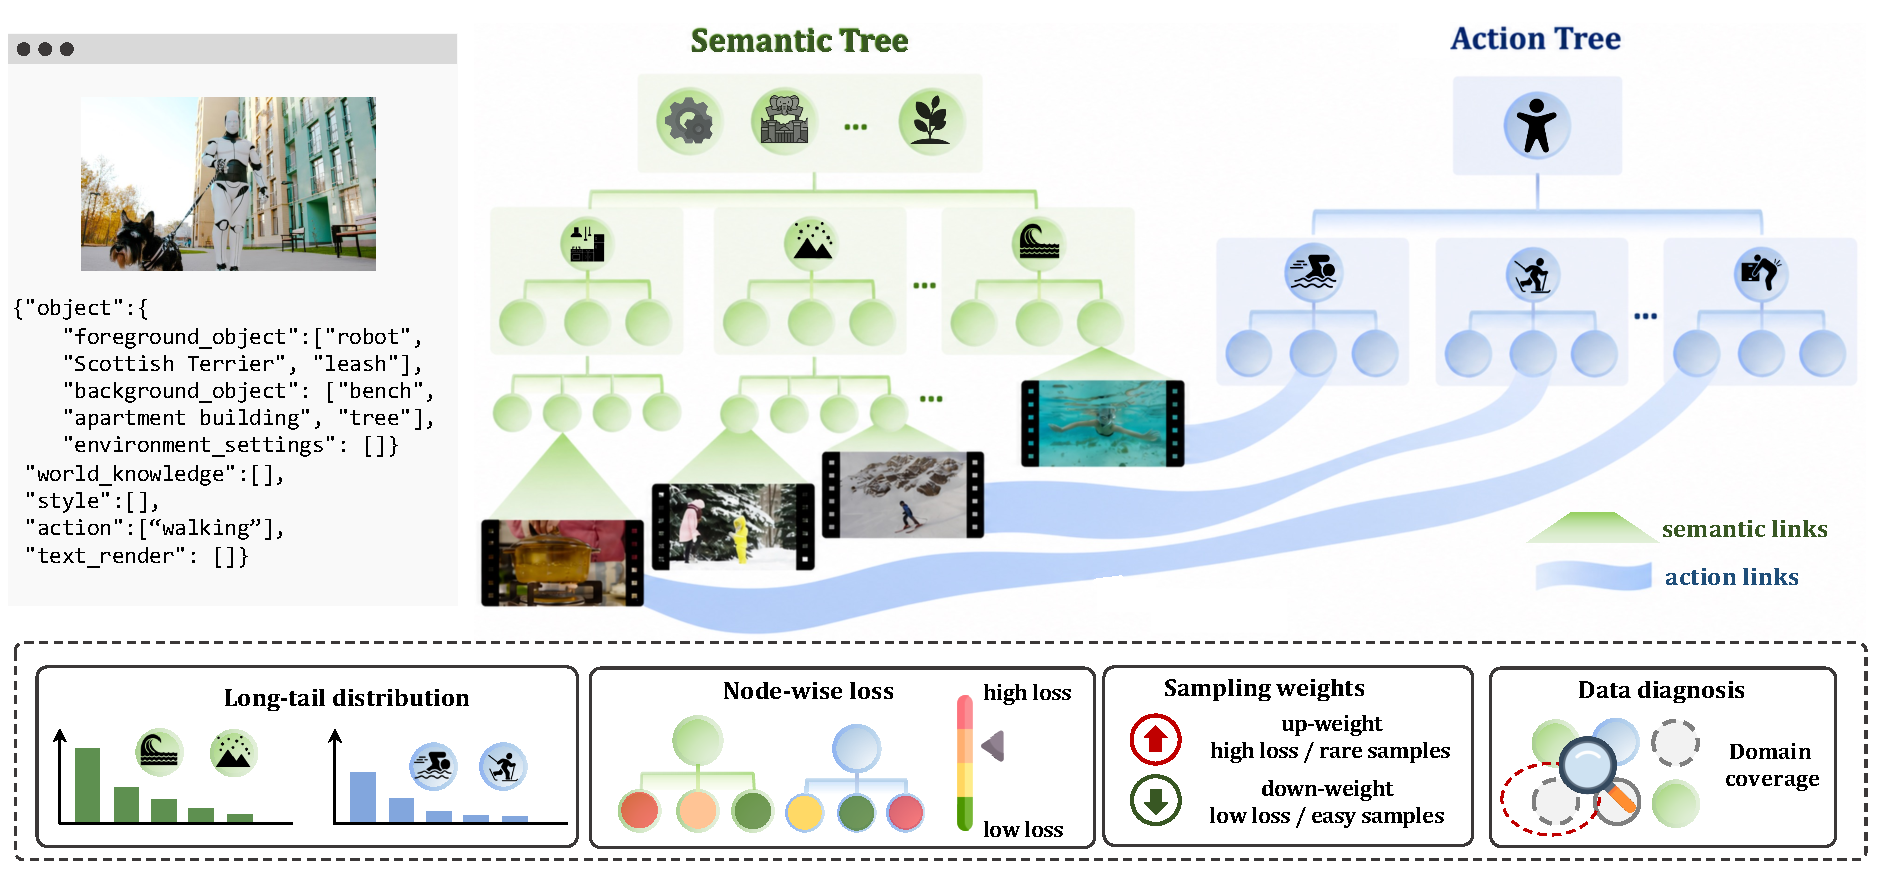
\includegraphics[width=\linewidth]{figures/world_knowledge_graph/world_knowledge_graph_light.pdf}
\caption{\textbf{World-Knowledge Topological Graph.} Structured tags from the Data Profiling Engine link each sample to a semantic tree of visual concepts and, for videos with actions, to an action tree of dynamic behaviors. The graph serves as a control surface for data curation: node statistics and training-feedback signals are used to up-weight rare or difficult concepts, down-weight saturated easy modes, and identify under-covered domains for targeted data expansion.}
\label{fig:world_knowledge_graph}
\end{figure}

\subsection{World-Knowledge Topological Graph}

To make data curation distribution-aware rather than quality-aware only, we construct a World-Knowledge Topological Graph~\cite{cai2025z} that organizes samples along two complementary axes: a semantic concept tree and an action tree.
The semantic tree is shared by images and videos, providing a common vocabulary for objects, scenes, visual styles, and world-knowledge entities.
The action tree is attached only to video samples and captures the dynamic behaviors that are especially important for video pre-training, such as object manipulation, sports, daily activities, and human gestures.
Together, the two views allow us to query not only what appears in a sample, but also what happens in it.

\noindent\textbf{Semantic Concept Tree.}
We first extract semantic tags from the Data Profiling Engine, including foreground and background objects, environment settings, world-knowledge entities, styles, and rendered text (\cref{fig:world_knowledge_graph}).
Directly embedding these raw tags is unreliable because many tags are sparse, ambiguous, or dominated by proper nouns and domain-specific terms.
We therefore expand each tag with a short textual introduction that describes its visually grounded meaning, and then embed the concatenation of the tag and its introduction.
The resulting representation is clustered together with frequently used Wikipedia concepts~\cite{wikidump,Page1999ThePC} to form a large hierarchical inventory.
This hierarchy contains $50{,}000$ fine-grained leaf concepts and $1{,}000$ intermediate visual categories.
At lower levels, embedding-based clustering~\cite{vo2024automatic} provides high coverage and scalability.
At the top level, however, purely automatic clustering tends to disagree with human perceptual granularity; for example, visually similar categories may be separated by ontology names, while visually distinct categories may be merged because their text descriptions are semantically close.
We therefore use an LLM-assisted \textbf{Discover--Classify--Consolidate} procedure to merge the $1{,}000$ intermediate categories into $25$ visually coherent top-level groups.
The discovery stage proposes an initial flat taxonomy from representative categories, the classification stage assigns all intermediate categories while allowing bounded new-bucket proposals, and the consolidation stage merges overlapping buckets, renames unclear buckets, and absorbs under-populated ones.
This produces a human-aligned tree in which each sample is assigned to a fine-to-coarse semantic path.

\noindent\textbf{Action Tree.}
For videos, we additionally construct an action tree from the action tags produced by the profiler.
Because raw action tags are short, noisy, and redundant, we first normalize their surface forms and then expand each tag with a short VLM-generated description grounded in representative video snippets.
We embed the concatenation of the action tag and its description, and cluster the resulting representations into canonical action nodes.
This description-augmented clustering reduces ambiguity in short action phrases while grouping visually similar motion patterns.
After clustering, we apply lightweight review and correction to high-frequency or ambiguous nodes, and discard unreliable long-tail actions.
This produces several hundred canonical action nodes covering manipulation, human gestures, sports, and daily activities.
All samples are indexed by their semantic paths, while videos with reliable action annotations are additionally linked to one or more canonical action nodes, giving us a joint semantic-action profile.

\noindent\textbf{Distribution-Aware Sampling and Data Diagnosis.}
The graph is used as a control surface for the late-stage data curriculum.
During challenge-focused continual training, we up-weight rare or difficult semantic and action nodes, especially those related to manipulation, physical contact, and long-tail human activities, while down-weighting over-represented generic video nodes.
Beyond static graph statistics, we further close the loop with training feedback from the earlier pre-training stages.
After the first two stages, we aggregate the denoising loss by semantic nodes and, for video samples, by action nodes, obtaining a node-aware estimate of data difficulty that informs the sampling weights in subsequent stages.
Because every node maintains sample counts and representative examples, the graph also exposes coverage holes: missing actions and under-represented object categories.
We use these signals to guide targeted data acquisition and to rebalance the training mixture, improving long-tail diversity without blindly increasing corpus size.

\subsection{Dense Structured Captioning} \label{subsec:dense_captioning}
Following FIBO~\cite{gutflaish2025fibo}, which shows that training on long structured
captions substantially improves prompt adherence and controllability, we
annotate all training data with dense structured JSON captions. Our captions
cover four types of data---images, videos, VLA videos, and egocentric
videos. All four types share the same schema: video, VLA, and egocentric
captions simply add a few extra fields on top of the image schema.
\begin{itemize}
  \item \textbf{Image captions.} Each image caption has four parts: (1) a
  comprehensive description of the whole image; (2) a set of camera tags
  (color tone, shot size, shot angle, lens type, composition,
  light quality, and light source),
  each chosen from a fixed set of values; (3) an optional world-knowledge
  list for named entities that appear in the image; and (4) a list of
  prominent elements. For every element, the caption describes its location,
  relative size, shape and color, texture, relationship to other elements,
  and orientation. If the element is a person, the caption also describes
  pose, gender, skin tone, expression, and clothing; if it is a group of repeated objects, the
  caption marks it as a cluster and gives a rough count.
  \item \textbf{Video captions.} Video captions add temporal information on
  top of the image schema. The global description is written in two parts:
  what happens in the scene, and how the camera moves. In addition, every
  prominent element carries a list of timestamped actions, e.g., a hand
  enters the frame during $[2.67s, 3.67s]$ to place a food item. The caption
  therefore tells the model not only what is in the video, but also who does
  what, and when.
  \item \textbf{VLA captions.} Robot-manipulation videos use the same video
  schema. Robotic arms and grippers are described as prominent elements like
  any other object, and their timestamped actions split each episode into
  clear phases, e.g., moving down to grasp, opening the gripper to release,
  and retracting. Gender and skin-tone fields are dropped for this data.
  \item \textbf{Egocentric captions.} First-person videos also use the video
  schema. The camera-movement field describes the wearer's head and body
  motion, and the wearer's hands are annotated as prominent elements, with
  timestamped actions describing how they interact with objects. Gender and
  skin-tone fields are likewise dropped.
\end{itemize}
One example caption for each data type is provided in~\cref{app:caption}.

\subsection{Caption Rewriter} \label{subsec:caption_rewriter}
The generator is trained conditionally on the dense structured captions described in~\cref{subsec:dense_captioning}---which are lengthy, attribute-rich, JSON-formatted descriptions. During inference, however, users typically provide brief, free-form prompts. To bridge this train--inference distribution gap, we introduce a \emph{Caption Rewriter} that decomposes prompt expansion and formatting into a two-stage pipeline, avoiding the unreliability of a single-step mapping model.

In the first stage, \textbf{Expand}, a zero-shot large language model (e.g., Qwen3.6-27B~\cite{qwen3.6-27b}) processes the user prompt into a compact, action-centric natural-language description (under a thousand characters). This stage intentionally generates a concise, non-enumerative description that omits overly specific fine attributes---such as texture, exact colors, relative sizes, and precise camera parameters---which are highly prone to hallucination. The second stage, \textbf{Map}, utilizes a Qwen3.6-27B fine-tuned with LoRA~\cite{hu2021lora} to transform this intermediate prose into the final structured JSON caption. Although the Map stage populates the complete schema, it operates under a strictly \emph{bounded completion} constraint: it must preserve all explicit information from the prose verbatim (including scene layout, subjects, timestamped actions, and named entities) and is only permitted to plausibly impute low-risk missing fields. This strategy confines potential hallucinations and allows the two-stage rewriter to produce significantly more reliable and better-structured captions than a single model tasked with expanding and structuring a prompt simultaneously.

Both stages seamlessly support text-to-video (T2V) and text-image-to-video (TI2V) generation. For TI2V, a conditioning first frame is provided as the $t{=}0$ ground truth, ensuring the visual appearance adheres strictly to the image while motion dynamics follow the text. Additionally, a target duration is appended to every prompt to constrain all predicted action timestamps to fall within the video's duration.

\subsection{Data Curriculum} \label{subsec:data_curriculum}
Building upon the curated corpus, we organize the training data into a five-stage curriculum aligned with the progressive pre-training schedule (\cref{sec:training}); here we focus on how the data itself evolves across these stages. The modality mix and per-source composition shift systematically---from low-resolution (192p) image-only data, through joint image--video data with embodiment-rich footage at increasing resolution, to a small high-quality video refinement set. The cascaded refiner (\cref{sec:method}) is trained separately on a high-quality 1080p subset of this corpus.~\cref{fig:data_curriculum} summarizes how the modality mix and per-source proportions evolve across the five stages.

\begin{figure}[t]
\centering
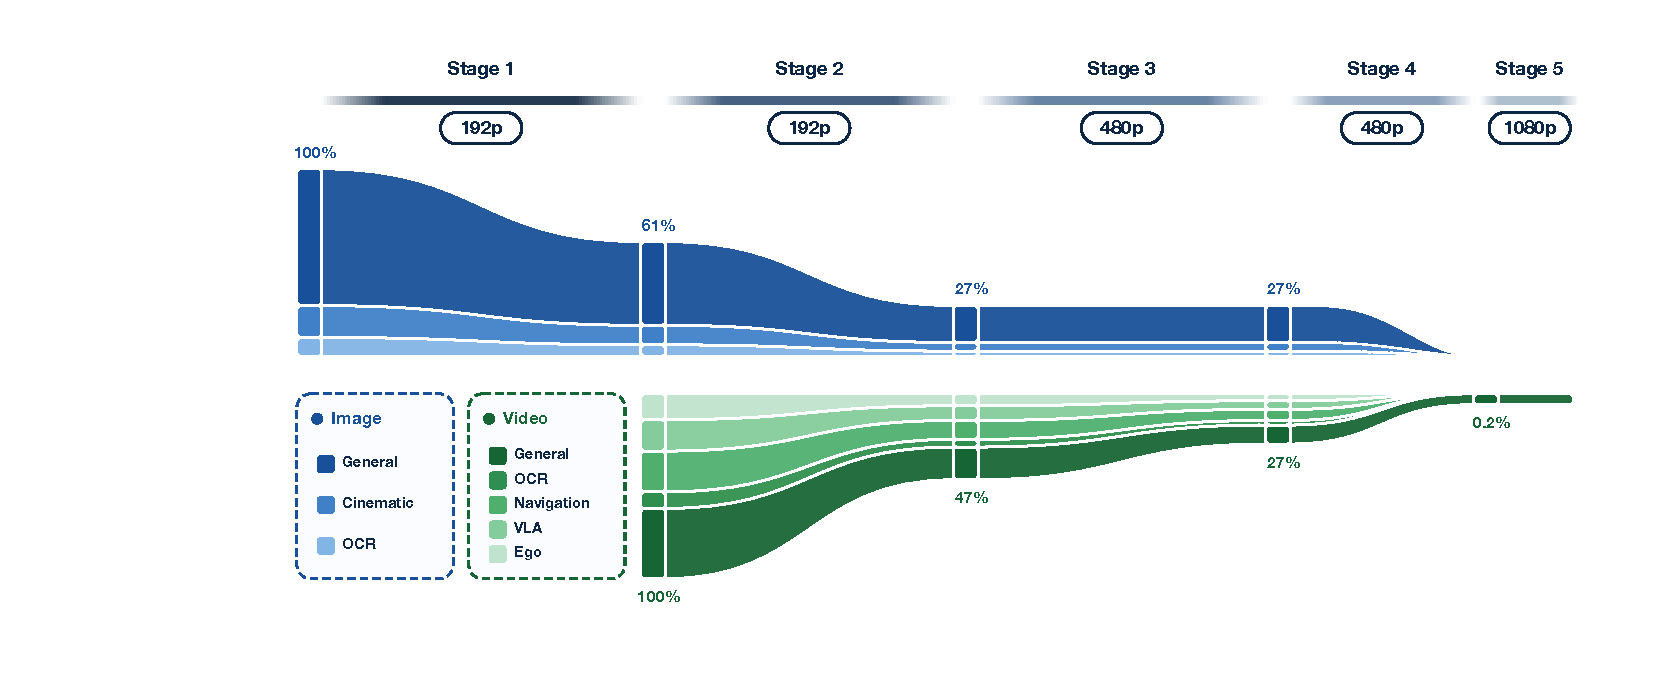
\includegraphics[width=\linewidth]{figures/data_curriculum_flow/data_curriculum_flow.pdf}
\caption{\textbf{Data curriculum across the five progressive pre-training stages.} The image stream (blue) and video stream (green) are decomposed into their constituent sources, with band width indicating each source's relative proportion; percentages denote the fraction of data retained at each stage relative to the modality's initial pool.}
\label{fig:data_curriculum}
\end{figure}

\noindent\textbf{Stage 1: Curated low-resolution image pool.}
The initial stage trains exclusively on 192p images, retaining the samples that pass aesthetic-quality and minimum-resolution filters while rigorously discarding the lowest-tier content.

\noindent\textbf{Stage 2: Video introduction and source expansion.}
Stage 2 introduces video content alongside images at a matching 192p resolution: a large corpus of video clips joins a quality-tightened, smaller pool of images. Video clips are admitted through a combination of resolution, aesthetic, and motion filters; notably, the motion criterion integrates a geometry-grounded tracking signal with a VLM-based motion assessment to robustly filter out near-static clips. Crucially, this stage marks the injection of over 70{,}000 hours of embodiment-oriented footage into the corpus---robot manipulation (VLA) spanning real-robot, simulated, open-source, and third-person perspectives across both humanoid and quadruped platforms, together with navigation and egocentric video---alongside text-rich video. Concurrently, the image filters are tightened to enforce higher aesthetic standards, a strict minimum resolution, and freedom from color cast, noise, and blur.

\noindent\textbf{Stage 3: Higher-resolution re-filtering.}
Stage 3 scales both the video and image streams to 480p, tightening the corresponding aesthetic and motion criteria proportionally; the higher-resolution bar substantially narrows the admitted data in both modalities. We purposefully retain high-motion video to strengthen coverage of dynamic content, while holding the image stream to the rigorous quality gates established in Stage~2.

\noindent\textbf{Stage 4: Challenge-focused rebalancing.}
At the same 480p resolution, this stage employs source-aware curation to align the corpus with the demands of embodied intelligence. Abundant general and curated videos are subjected to stringent quality standards covering resolution, aesthetics, clarity, motion, and freedom from artifacts such as watermarks, whereas scarce yet high-value embodiment sources, including manipulation, navigation, egocentric footage, and benchmark datasets, undergo only minimal filtering to maximize their coverage. This deliberate asymmetry trades redundant general footage for the long-tail, action-centric data that is paramount for embodied intelligence, yielding a mixture far more embodiment-heavy than the raw source counts would suggest.

\noindent\textbf{Stage 5: High-quality refinement subset.}
The final stage is a small, high-quality video refinement set at 1080p, used to train the cascaded refiner (\cref{sec:method}): a curated subset drawn from the general source, with samples held to the strictest aesthetic, resolution, and technical-quality bars, and only a tiny fraction (well under 1\% of the initial video pool) retained.

